\documentclass[psfig,preprint]{aastex}
\begin{document}

\title{A SHORT UNIX PRIMER}
\author{Carl Heiles  \\ \today}

%\author{Carl Heiles \altaffilmark{1} \\ \today}
%\altaffiltext{1}{Based on earlier versions by Anthony Truong and
%Jennefer King.}

\tableofcontents

\section{DIRECTORIES AND SUBDIRECTORIES} \label{directories}

For experienced programmers the hardest thing about computing is keeping
things organized. You end up with thousands of files and need to keep
them in functional categories. You do this by creating appropriate
directories and keeping your files there. 

\subsection{The Directory Tree}\label{thedirtree}

For example, when you begin a project, such as an experiment, you should
create a directory for that project---and that directory needs an
appropriate name. For the lab class, you might name the directory
{\tt lab1}. For this project
you will have several activities: taking data, analyzing data, and
writing the lab report. So under the {\tt lab1} directory you might
create three subdirectories entitled {\tt data}, {\tt idl}, and {\tt
  tex}. You have created a little directory tree!

This tree lives under your main directory, called your {\tt home}
directory. The name of your home directory is your login name, which is
(probably) the first letter of your first name plus the first seven
letters of your last name. Your home directory has, as its root, a
system directory called {\tt home}. Thus, {\tt home} is the origin of
all users' directories. Your personal tree has, as its origin, your home
directory. When you create the lab1 directory under your home directory,
you've created a new branch of your directory tree.


\begin{figure}[h!]
\begin{center}
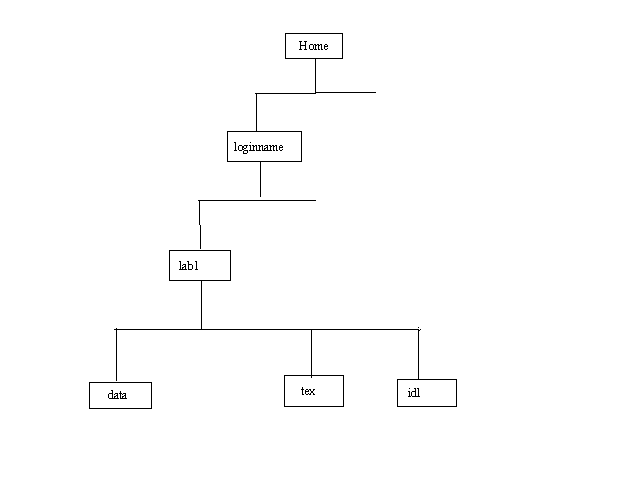
\includegraphics[scale=0.4]{dirtree.png}
\end{center}
\caption{The directory tree described in the text. 
\label{dirtree}}
\end{figure}

Figure \ref{dirtree} shows the schematic structure of this directory
tree. It is impossible to overemphasize the importance of your creating
and maintaining a sensible directory tree.

\subsection{Working with Directories}

We have configured our system so that the prompt contains the name of
the current directory. Another way to determine where you are is with
the Linux/UNIX command {\tt pwd} (short for ``Present Working
Directory''). Try it!

The most important commands relevant to directories include: \begin{enumerate}

\item To see a listing of the files and subdirectories of the present working
directory (pwd), use
the {\tt ls} command.  It has some useful
options. One of my favorite combinations of options is {\tt ls -lrt}:
the {\tt l} means ``long listing format'', the {\tt t} means ``time
order'', and the {\tt r} means ``reverse order''---so this lists all
files in reverse time order so that the most recent file appears as the
last line of the list. You can also use the {\tt *} character as a
wildcard: for example, {\tt ls *ps} lists all files with the suffix {\tt
    ps} (these are usually PostScript files). 

\item To change to a directory, e.g.\ the {\tt tex} directory under {\tt
  lab1}, type {\tt cd /home/loginname/lab1/tex}. Or, shorter: \verb$~$
  stands for your home directory, so you can type
  \verb$cd ~/lab1/tex$. Or, if your present working directory (pwd) is
  {\tt lab1}, you can type just {\tt cd tex}.


\item To create a new directory, e.g.\ a directory called {\tt monday}
  under {\tt data}, type \\ \verb$mkdir ~/lab1/data/monday$. Or, if your
  pwd is \verb$~/lab1/data$, you need only type {\tt mkdir monday}. If
  you want to eliminate (remove) a directory, get rid of all the files
  and type {\tt rmdir monday}.

\item To copy a file from one directory to another, e.g.\ the file {\tt
  carl} from \verb$~$ to \verb$~/lab1/idl$, type
  \verb$cp ~/carl ~/lab1/idl$. You end up with two copies of the file. You
  can instead move the file using {\tt mv}. To remove a file, use {\tt
  rm}.

We have defined the following options for these commands:
\begin{enumerate}

\item For {\tt cp}: {\tt cp -ip}. The {\tt i} means ``inquire before
  overwriting a file of the same name''; once you overwrite the original
  version, it's gone! the {\tt p} means ''preserve the original time
  information about the file''; otherwise, it would tag the copied file
  with the current time.

\item For {\tt mv}: {\tt mv -i}. As above. inquire!

\item For {\tt rm}: {\tt rm -i}. Ask to confirm your intention to
  eliminate the file. Once it's gone, it's gone---there's no
  ``wastebasket''. 
\end{enumerate}

\end{enumerate}

\subsection{Permissions for Directories and Files} \label{perm}

Permissions determine who has access. You might want your data to be
accessible by everybody, for reading, but you probably don't want other
people writing over your data!  And you shouldn't want your lab writeup
to be accessible by anybody, either reading or writing---you don't want
to facilitate plagiarism! And it makes sense to keep all your love
letters in a separate directory that isn't accessible in any way by
anybody else---including their recipient(s)!

You set permissions with {\tt chmod}.  Permissions recognize three
classes of people: {\tt u} ({\it user}---yourself!), {\tt g} ({\it
group}---that's usually all the users of {\tt ugastro}), and {\tt o}
({\it other}---everybody else, {\it including} somebody in Timbuktu who
happens to crash into our system). Note that {\it group} is essentially
like {\it other}---almost everybody! Each class can have three
permissions: {\tt r} (read permission), {\tt w} (write permission), and
{\tt x} (execute permission).  {\tt chmod} allows you to add, take away,
and set exactly permissions for different users with the operators ({\tt
+, -, =}).

Suppose, for your data subdirectory, you want read permission for
everyone and write permission only for yourself. To grant the read
permissions to {\it group} and {\it other}, get into the directory above
{\tt data} (that's {\tt lab1}) and then type {\tt chmod go+rx data}; to
eliminate the write permissions, {\tt chmod go-w data}. To check your
work, do a long listing of the directory ({\tt ls -l data}). On your
screen, it would write

\noindent \verb$drwxr-xr-x 1 heiles bin 10 2007-01-20 17:58 data/$

\noindent Translation: The first character, {\tt d}, means it's a
directory. The next three specify the permissions for the user (that's
you): {\tt rw} means you have read, write privileges, and the {\tt x} means
you can access the directory. The next set of three characters {\tt
  r-x} is for
the group (all your classmates); the final set of three characters {\tt
  r-x} means that everybody can read and access the directory contents,
but can't write into it.

For your love letter directory (called {\tt love}, you'd want {\tt chmod
  go-rwx love}

Permissions apply slightly differently to directories and files: \begin{enumerate} 

\item {\it Directories.} In order to access any file in a
  directory---even to obtain a listing of the files with the {\tt ls}
  command---the person needs {\it execute} permission. The read and
  write permissions are as you'd expect.

\item {\it Files.} Most files don't need execute permission. By
  default, when you create a file, it has read/write permissions for you
  and read for the other two classes.

\end{enumerate}

\section{OTHER ASPECTS\dots}


\subsection{Command-Line Editing in Linux/UNIX, Emacs, and IDL}

\label{keycommands}

One of the joys of Linux/UNIX is command-line editing using keystrokes. We have
configured IDL to use the same keystroke commands; Emacs already does so.
The most important command-line editing commands are:

\begin {tabbing}
{\bf arrow keys} \hspace{0.8in} \= move the cursor as you'd expect. \\
{\bf Ctrl-d} \> deletes the character under the cursor. \\
{\bf Backspace} \> deletes the character behind the cursor. \\
{\bf Ctrl-e} \> moves the cursor to the end of the line. \\
{\bf Ctrl-a} \> moves the cursor to the beginning of the line. \\
{\bf Ctrl-k} \> deletes the the rest of the line.
\end{tabbing}

\noindent Sometimes, when command-line editing, you inadvertently hit
{\bf Ctrl-s}; this prevents the cursor from responding to your
keystrokes. If you encounter this condition, type {\bf Ctrl-q}, after
which things will work normally again.

	In X windows, you can customize any X window to your desires
(e.g.\ fontsize) by putting the cursor on the window, holding down the
CTRL or SHIFT key and, simultaneously, holding down a mouse button; each one
provides different options.  If you are using KDE or Gnome, the details
differ. 

\subsection{Aliases}\label{short}
	
	Aliases are shortcuts that you can use in place of typing out a
long command over and over again.  You can define an alias on the
command line; alternatively, if you want to define it permanently, you
can define it by editing your {\tt .cshrc} or {\tt .aliasfile} file
(which reside in your home directory).

	Here's an example. Suppose that you want to force UNIX to check
whether it will overwrite a file when you use the {\tt mv} command and,
also, to ask you about it. To do this,
you use the {\tt -i} option, and you redefine the command {\tt mv} by
typing

\noindent {\tt alias mv "mv -i"}

\noindent If you type it in a window, it will apply henceforth to that
window alone.  

We have included this definition in your {\tt .aliasfile}, which
resides in your home directory and is automatically invoked whenever
you open a new terminal window---because your {\tt .cshrc} file invokes
your {\tt .aliasfile}. 

You can check the definition of the alias for {\tt mv} by typing

\noindent {\tt which mv}

Finally, you can bypass any defined alias by using a backslash. For
example, \verb$\rm carl$ invokes the {\tt rm} command without the {\tt
-i} option that is defined in your {\tt .aliasfile}, which means\dots it
removes the file {\tt carl} {\it without asking}. Using {\tt rm}, {\tt
  cp}, or {\tt mv} without the {\tt -i} option is {\it dangerous}: Once
a file has been overwritten or deleted, it's gone for good!

\subsection{Piping, etc: $|, >, <$}\label{help}

	Piping (\verb$|$)  directs the output of a command to the next succeeding
command.  For example,

\noindent \verb$ls | grep /$

\noindent directs the output of the listing command to {\it grep}, which
here selects all names containing the string ``/''; those are
directories, so this gives a list of directories just under the current
directory. 

	Normally the result of a UNIX command is written to the terminal
for you to see. However, you can direct the output elsewhere. For
example, 

\noindent {\tt more love1}

\noindent prints the file {\tt love1} on your screen, while

\noindent \verb$more love1 > love2$
 
\noindent creates the file {\tt love2} and writes the content into it.

	Normally the input to a UNIX command is expected to be from the
terminal. However, you can get the input from elsewhere. For example, 

\noindent \verb$mail heiles < complaint.txt$

\noindent uses the file {\tt complaint.txt} as input to the command {\tt
  mail}, which means that it mails the file {\tt complaint.txt} to
  heiles; try it! (Do you think he pays any attention to his mail? Do
  you think it will do any good???)

\subsection{Remote Logging In}\label{remote}

	You can log in from home {\it if} your computer has the secure
login software, called {\tt ssh}. 
If you have Linux, type {\tt ssh ugastro.berkeley.edu}

If you're logging in from home on an (ugh!) Windows machine, you need to
be able to use X windows; for this, run the program {\tt exceed} before
logging in. You can get such software from the CD {\it Connecting @
Berkeley}, available for free from the big U.


\eject

\section{COMMON COMMANDS}\label{commands}
\vspace{-0.2in}

\begin{tabbing}
%\textit{passwd} \hspace{1.6in} \=  Useful for changing your account password. \\
\textit{man commandname} \hspace{0.7in} \= Gets voluminous (usually overly so) info for you on a specific command. \\
\textit{apropos topic} \> Tells which commands are
relevant to the {\it topic}. \\
\textit{pwd} \> Shows your ``present working directory''. \\
\textit{cd dirname} \> Moves you into the subdirectory, below your 
present directory. \\
\textit{cd ..} \> Moves you out of a subdirectory into the directory above
it. \\
\textit{cd -} \> Moves you to previous directory you were in. \\
\textit{mkdir dirname} \> Creates a subdirectory named \textit{dirname}. \\
\textit{rmdir dirname} \> Removes a subdirectory named \textit{dirname}. \\
\textit{rm filename} \> Removes a file named \textit{filename}; it must
be empty. \\ 
\textit{cp file1 file2} \> Copies the contents of \textit{file1} into 
\textit{file2}. You are left with two files. \\
\textit{mv oldfile newfile} \> Moves (or renames) \textit{oldfile} as 
\textit{newfile}. \\
\textit{cat file1 file2 $>$ fileboth} \> Concatenates {\it file1} and {\it
file2}, writing them into the new {\it fileboth}. \\
\textit{which cp} \> Tells the current definition of {\it cp} ({\it which}
works for any command); \\
\textit{history} \> Gives a numbered list of the previous commands you've
typed; \\
\> typing {\bf !number} repeats that command. \\
\textit{!!} \> Repeats the previous UNIX command. \\
\textit{find dirname -name filename} \> finds all files with {\it
filename} in and under the directory with {\it dirname}. \\
\textit{find dirname -name '*love*'} \> Finds all files whose names 
contain the string ``love''. \\
\textit{ls -lrt} \> Lists the files and subdirectories 
in the present directory. \\
\>The {\it -lrt} gives a long format in reverse time order.\\
\textit{ls -lrt $|$ grep /} \> Pipes the output to {\it grep}, which \\
\> selects only those names containing ``/'' (which are directories). \\
\textit{du -h dirname} \> Tells the disk space used by everything in dirname. \\
\>The ``h'' means in ``human units''. \\ 
\>Also handy for giving the directory tree structure. \\

\textit{df -k} \> Tells kilobytes used and available on all
disks. (``-h'' works here too!)\\
\textit{grep -il text file} \> Searches the \textit{file} for occurrences of
the string \textit{text} \\
\> The {\it -i} ignores capitalization and {\it l} lists only the filename.\\
\textit{lp filename} \> Prints the contents of \textit{filename}. \\
\textit{enscript filename} \> Fancier print than {\it lp}. \\
\textit{less filename} \> Shows you the contents of the file named 
\textit{filename} one screen at a time; \\
\> more flexible than {\textit more}. \\
\textit{tail -40 filename} \> Shows you the last 40 lines of the file
{\it filename}. \\
\textit{lpq} \> Displays the print queue. \\
\textit{cancel jobnum} \> Removes the \textit{jobnum} in the print
queue. You must own the job \\

\textit{top} \> Shows CPU usage, etc, for jobs on your machine. \\
\textit{ps -u username} \> List the programs that \textit{username} is
currently \\
\>  running on the machine you are logged onto. \\
\textit{kill processnum} \> Kills the process listed with
\textit{processnum}. You must own the process \\
\end{tabbing}
	



\end{document}


